\documentclass[main]{subfiles}
%%\documentclass[preprint,12pt,authoryear]{elsarticle}
\usepackage[ruled]{algorithm2e}
%\RequirePackage{natbib}
\usepackage{amsmath}
\usepackage{varwidth}
\usepackage{amssymb}
\usepackage{mathtools, cuted}
\usepackage{amsthm}

\newtheorem{theorem1}{Special Theorem}
\newtheorem{definition}[theorem1]{Definition}
\newtheorem{proposition}[theorem1]{Proposition}
\newtheorem{theorem}[theorem1]{Theorem}
\newtheorem{example}[theorem1]{Example}
\newtheorem{lemma}[theorem1]{Lemma}

\usepackage{caption}
\usepackage{subcaption}
\usepackage{booktabs}
\usepackage{graphicx}

\usepackage{tikz}
\usetikzlibrary{arrows,shapes,positioning,shadows,trees}
\newcommand{\indep}{\rotatebox[origin=c]{90}{$\models$}}
\tikzset{
  basic/.style  = {draw, text width=2cm, drop shadow, font=\sffamily, rectangle},
  root/.style   = {basic, rounded corners=2pt, thin, align=center,
                   fill=green!30},
  level 2/.style = {basic, rounded corners=6pt, thin,align=center, fill=green!60,
                   text width=8em},
  level 3/.style = {basic, thin, align=left, fill=pink!60, text width=6.5em}
} 

\newcommand{\todo}[1]{{\color{blue} #1 }}

\begin{document}

\begin{frontmatter}

%\title{A Flexible Framework for Conformal Predictions on Multiple Non-disclosed Datasets}
\title{Aggregating Predictions on Multiple Non-disclosed Datasets using Conformal Prediction}

\author[label1]{Ola Spjuth}
\ead{ola.spjuth@farmbio.uu.se}
\author[label2]{Lars Carlsson}
\ead{Lars Carlsson <dr.lars.carlsson@gmail.com}
\author[label1]{Niharika Gauraha}
\ead{niharika.gauraha@farmbio.uu.se}


\address[label1]{Department of Pharmaceutical Biosciences \\
       Uppsala University\\
       Uppsala, Sweden}
\address[label2]{Department of Computer Science, \\Royal Holloway, University of London, \\Egham Hill, Egham, Surrey, United Kingdom}


\begin{abstract}
The flexible framework for machine learning algorithms called conformal prediction, provides region predictions with guaranteed confidence under mild conditions. %error rate. Transductive version of conformal predictors have been proven to be valid and more information efficient. 
In this paper, we extend the basic conformal prediction framework to handle %conformal predictions combining results from 
multiple data sources that do not require sharing of data.
We propose to aggregate conformal predictions from multiple sources, where transductive conformal predictors are applied on the data sources independently, and their individual predictions are aggregated to form a single prediction on a new example. We demonstrate the method on several data sets, and show that the proposed method produces valid and efficient predictions. We also study the effect of pooled data size, number of data sources, size of each source has on predictions.
\end{abstract}
\begin{keyword}
%% keywords here, in the form: keyword \sep keyword

%% PACS codes here, in the form: \PACS code \sep code

%% MSC codes here, in the form: \MSC code \sep code
%% or \MSC[2008] code \sep code (2000 is the default)
Conformal Prediction \sep aggregated predictions \sep non-disclosed data
\end{keyword}

\end{frontmatter}

\section{Introduction}
%it is not uncommon to have multiple sources of data .

The increasing volumes of data generated in virtually all scientific and industrial domains presents formidable challenges to store and analyze. Of particular interest is to make use of the information in statistical learning systems (predictive modeling). If data reside in multiple data sources, possibly in different databases or locations, the most common approach is arguable to collect all data intended for model building in a single location, such as a data warehouse or a file system, after which it is subjected to learning algorithms and subsequent predictions. However, if data is large or if the data owners do not allow such pooling of data, this strategy may not be possible. One example is in the pharmaceutical industry where large databases are available at companies, each holding results on e.g. chemical compounds tested against different endpoints in drug discovery projects. This information is valuable and sensitive for these companies, but at the same time there are occasions where companies would want to contribute to predictive models without disclosing the data to others, including pre-competitive initiatives and in interactions with CROs. There are approaches that have been developed towards integrated analysis that do not require sharing of original data, but there are limitations with these. For example, methods for integrated analysis of non-sensitive availability derived from original data has been developed~\cite{Spjuth:2016ly} but these are not suitable in machine learning contexts. Another example is dataSHIELD~\citep{Gaye:2014sf} which comprises a technically advanced computational infrastructure and uses distributed computing and parallelized analysis to enable joint analysis, but is does not support machine learning models. %\todo{CONFIRM THIS}
 
In this article we propose to improve predictions over different sources without explicitly sharing the data, by aggregating conformal predictions computed at individual locations. 
Basically, conformal predictors are confidence predictors that results prediction sets for all confidence levels. Thus, conformal prediction is a framework that complements the predictions of machine learning algorithms with reliable measures of confidence.
Transductive version of conformal predictors have been proven to be valid and more information efficient. In this paper, we extend the basic conformal prediction framework to handle multiple data sources and without sharing of data between sources. We propose to aggregate conformal predictions from multiple sources, where transductive conformal predictors are applied on the multiple data sources and their individual predictions are aggregated to form a single prediction on a new example.

The advantages of this approach of combining conformal predictions across multiple sources are two fold. 
Firstly, it is more a framework than a method, and it extends the existing framework of conformal prediction for multiple data sources, that do not require sharing of data. Secondly, combined analysis produces much more efficient predictions than individual analyses. This innovative framework is flexible in the sense it supports flexible number and sizes of data sources.

At a high level, our algorithm works as follows. Consider a binary classification problem, and suppose we have a training dataset $Z$ and an external test data $x$. The training data set is randomly and unequally split into K parts. For example, Let $Z = \{ z_1 , ..., z_n \} $ be the data set of $n$ observations, then we divide the dataset into $S_1, ..., S_K$ such that $Z = \bigcup_{i=1}^K S_i$, and $n = k_1+ ...+k_K$, where $k_i = |S_i|$. We compute p-values under TCP framework using the combined dataset  $(S_i,x)$ for each $S_i$. We have K p-values (for each class), now we aggregate (weighted) the k, p-values to obtain a final p-value for each class for the new example $x$. We repeat the process say $q$ times by varying number and sizes of the sources. The final analysis consists of analysing $q$ results which accounts for number as well as size of the data sources.

\begin{figure}[b!]
    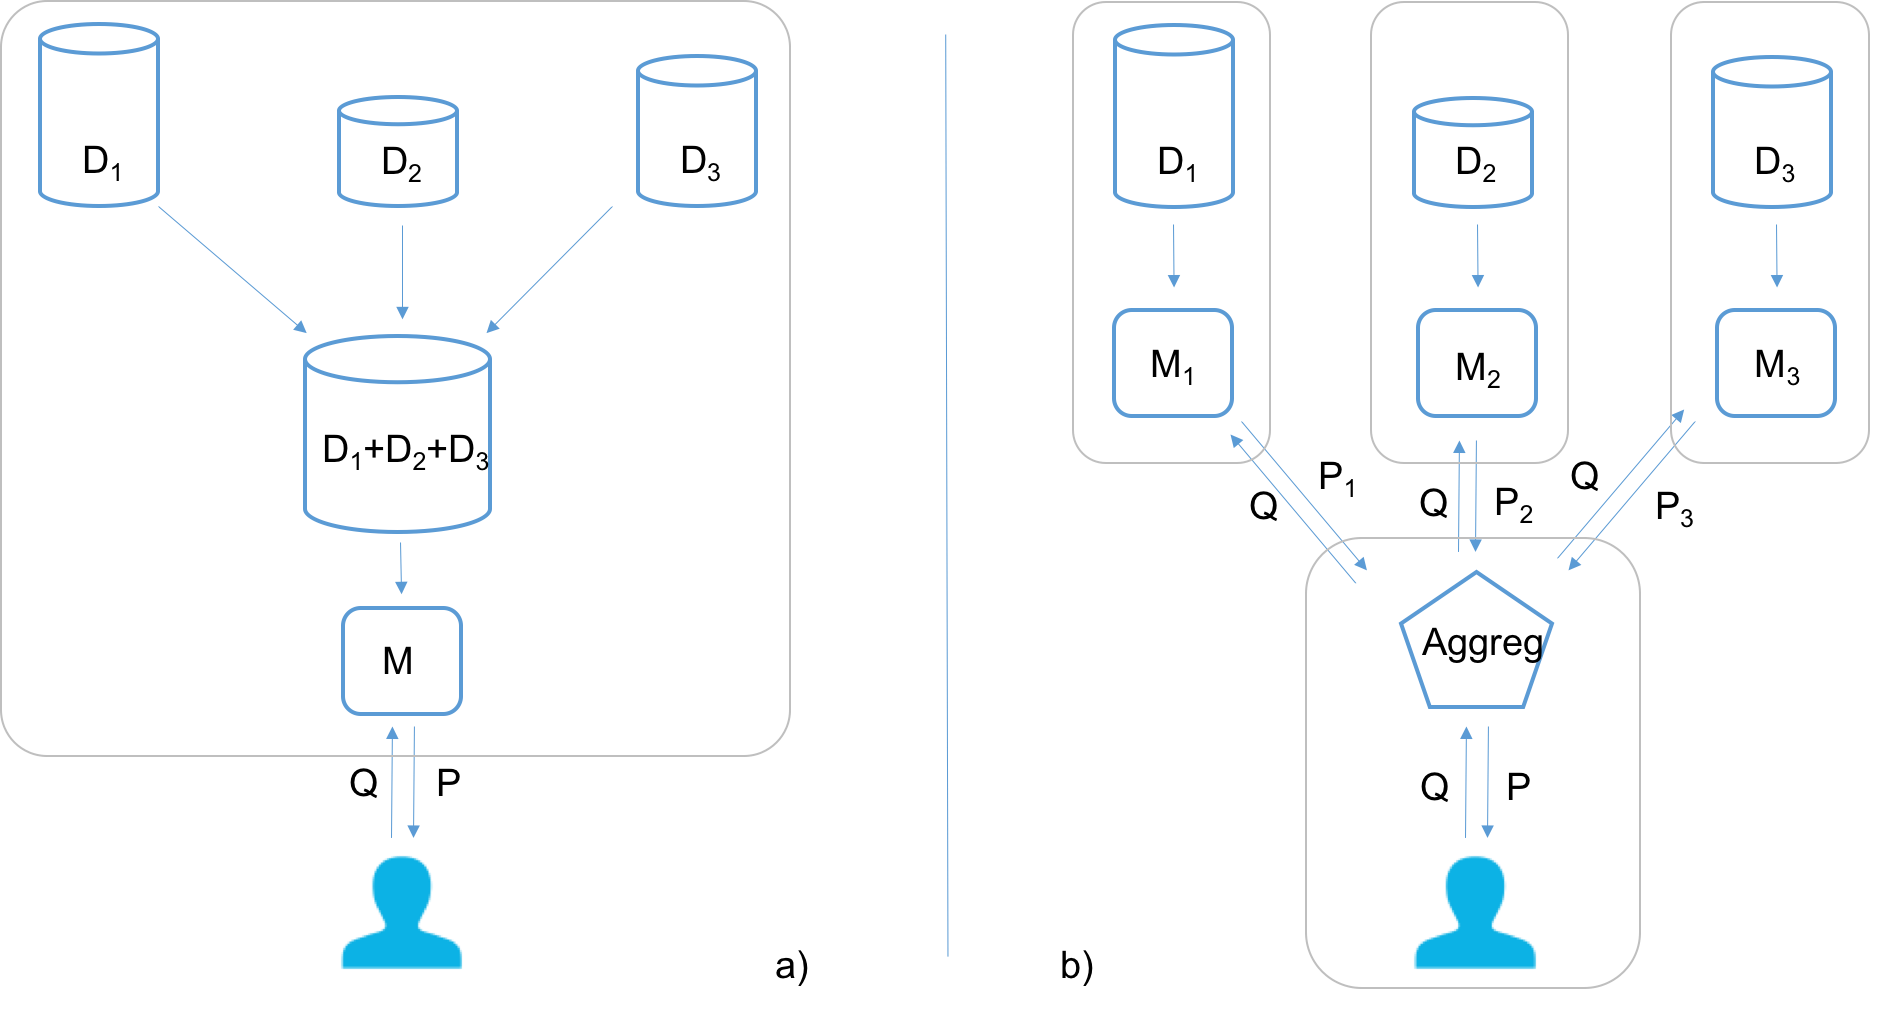
\includegraphics[width=0.95\textwidth]{images/fig-overview.png}
    \caption{\textbf{a}) The most common approach is to collect data from different data sources ($D_1-D_3$) into a single dataset, which then is used to train a model $M$ that can be used to make a prediction $P$ on a query object $Q$. \textbf{b)} The aggregated TCP approach implies that a model $M_n$ is trained at each data source $D_n$, and the query object Q is passed on to each model, and predictions $P_n$ are then aggregated to deliver the resulting prediction $P$. The gray wireframes are used to visualize the different actors taking part in the procedure independent of each other.}
  \label{fig:overview}
\end{figure}



%We illustrate the method using simulated and real data sets, and we show that the proposed method produces much more efficient predictions than individual analsys.

The contributions of this paper is summarized as follows:

\begin{enumerate}
\item to investigate if and how the number of data sources and size of the sources affect the aggregated efficiency and validity

\item to evaluate how good both ``aggregated equally partitioned" and ``aggregated randomly partitioned" perform when compared to the whole (pooled) data set.

\item to evaluate if and under what conditions aggregated TCP delivers acceptable results when compared to pooled data

%\item to show that the combined results are better (synergy) than the individual source p-values.


\end{enumerate}

The organization of the paper is as follows. In section 2, we introduce the background concepts and notation, used throughout the paper. In Section 3, we will introduce the concept of aggregating conformal predictions from multiple sources. In Section 4, we discuss the statistical properties of aggregated conformal predictions from multiple sources. In Section 5, we perform some numerical analysis on simulated and real datasets. Finally, in Section 6, the summary of the papery is provided.
%We have also included an appendix that reviews the most relevant aspects about TCP, ICP, CCP and ACP.\todo{do we really have to do this?}
\end{document}